The SLAC CRYO ASIC differs from the ``baseline'' three-chip design in that it combines the functions of an analog preamplifier, ADC and data serialization/transmission, for 64~wire channels, into a single chip.
It is based on a design developed for the nEXO experiment and differs from it only in the design of the preamplifier, which is modified to account for the higher capacitance of the DUNE wires compared to the small pads of nEXO.
FEMBs constructed using this chip would use only 2 ASICs compared to the 18 (8~FE, 8~ADC and 2~COLDDATA) neeeded in the baseline design.
This drastic reduction in part count may significantly improve FEMB reliablity, reduce power, and reduce costs related to production and testing. 

Figure~\ref{fig:cryo-architecture} shows the overall architecture of the CRYO ASIC, which will be implemented in 130~nm CMOS.
It comprises two identical, 32-channel blocks. 
The current signal from each wire is amplified using a preamplifier with pole zero cancellation and an anti-alias fifth-order Bessel filter applied. 
Provisions is also made for injection of test pulses. 
Gain and peaking time are adjustable to values similar to those of the baseline design.

\begin{dunefigure}
[Overall architecture of the CRYO ASIC.]
{fig:cryo-architecture}
{Overall architecture of the CRYO ASIC.}
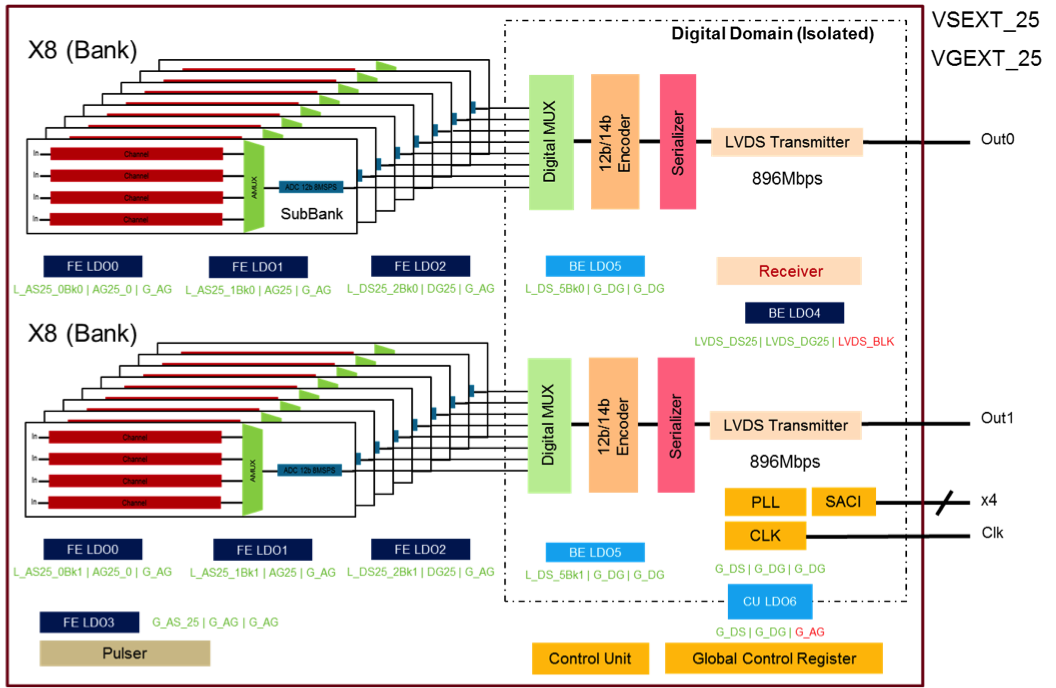
\includegraphics[width=0.8\textwidth]{tpcelec-cryo_schematic.png}
\end{dunefigure}

The ADC uses 8~MHz Successive Approximation Registration (SAR), so that four input channels are multiplexed onto a single ADC. The data serialization and transmission block employs a custom 12b/14b encoder, so that 32 channels of 12-bit, 2~MHz data can be transmitted with a digital bandwidth of only 896~Mbps, which is significantly less than the required bandwidth of the baseline, which is 1.28~Gbps.

One key concern with ``mixed signal'' ASICs is the possibility of interference from the digital side causing noise on the very sensitive preamplifier. 
Fortunately, there are well established techniques for ``substrate isolation'' described in the literature~\cite{yeh}, which have been successfully employed in previous ASICs produced by the SLAC group.% Figure \ref{fig:cryo-substrate} shows how substrate isolation is achieved. 

%\begin{dunefigure}
%[Depiction of the substrate isolation technique that allows combining analog and digital circuitry on the same CRYO ASIC.]
%{fig:cryo-substrate}
%{Depiction of the substrate isolation technique that allows combining analog and digital circuitry on the same CRYO ASIC.}
%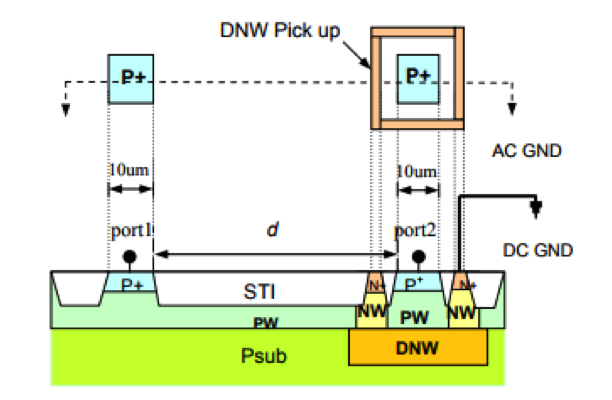
\includegraphics[width=0.6\textwidth]{tpcelec-cryo_substrate.png}
%\end{dunefigure}

The infrastructure requirements for a CYRO ASIC-based system are similar to those of the baseline option. However, in most cases, somewhat fewer resources are needed:
\begin{itemize}
\item{A single voltage is needed for the power supply. This is used to generate two supply voltages using internal voltage regulators.}
\item{The output digital bandwidth on each of the four lines in an FEMB is 896~Mbps. This is lower than the baseline option due to the custom 12b/14b encoder of the CRYO chip. }
\item{The warm interface is different. Only a single clock is needed (56~MHz) and the configuration protocol is the SLAC ASIC Control Interface (SACI)~\cite{SACI} rather than I2C.}
\end{itemize}

The first prototype of the CRYO ASIC is in the final design and simulation stages. Simulation-based studies have already been performed; at 0.8~\si{\micro}s peaking time and an input capacitance of 200~pF (similar to that expected in the DUNE far detector), the ENC is approximately 500e$^-$.  This noise level is similar to that expected with the baseline front-end and ADC ASIC design in LAr with the same input capacitance.  Submission to the ASIC foundry is imminent and the first protypes should be received by Summer 2018. They will first be tested in an existing test stand at SLAC. Subsequent tests are planned for a small test TPC at FNAL and on an APA in the ProtoDUNE-SP cold box; these test facilities are described in Section~\ref{sec:fdsp-tpc-elec-qa-facilities}.
